\section{Question 8}

    \subsection{Specify the Polling Server for this task set. Maximize server utilization, i.e., do the
    best server you can. Motivate your answer e.g. by a schedulability analysis}

        The task set will be scheduled with RM. To make sure the task set is schedulable with the extension of a PS, we have to make sure the following statement is true: $U_P + U_S <= (n+1)(2^{\frac{1}{n+1}} - 1)$ where $n$ is the number of tasks in the task set. 
        The following is the given task set:

        \renewcommand{\arraystretch}{1.4}
            \begin{figure}[H]
            \centering
            \begin{minipage}{0.5\textwidth}
                \begin{table}[H]
                \centering
                \begin{tabular}{|l|l|l|}
                    \hline
                    \textbf{Task}   & \textbf{T=D}  & \textbf{C}  \\ \hline
                    A               & 6             & 1           \\ \hline
                    B               & 8             & 2           \\ \hline
                    C               & 12            & 3           \\ \hline
                \end{tabular}
                \end{table}
            \end{minipage}%
            \caption{Task set}
            \label{fig:Q8tasks}
            \end{figure}
        \renewcommand{\arraystretch}{1.0}


        \begin{itemize}
            \item $U_P = \sum_{i=1}^{n} \frac{C_i}{T_i} = \frac{1}{6} + \frac{2}{8} + \frac{3}{12} = \frac{2}{3}$
            \item $\frac{2}{3} + U_S <= (3+1)(2^{\frac{1}{3+1}} - 1) = 0.757$
            \item $U_S <= 0.757 - \frac{2}{3} = 0.09$
        \end{itemize}

        The maximum $U_S$ is $0.09$ to make the task set schedulable with the extension of a PS. A PS which supports this $U_S$ is:
        \begin{itemize}
            \item $C_s = 9ms$
            \item $T_s = 100ms$
        \end{itemize}

    \subsection{The same question as above, but for Total Bandwidth Server}
        
        This time the task set will be scheduled using EDF. To make sure the task set is schedulable with the extension of a TBS, we have to make sure the following statement is true: $U_P + U_S <= 1$ where $U_S$ is the processor utilization factor of the TBS. $U_P = \frac{2}{3}$ as before and to make the statement true we have to make sure that $U_S <= 1 - \frac{2}{3} = \frac{1}{3}$. So the maximum $U_S$ is $\frac{1}{3}$ to make the task set schedulable with the extension of a TBS.

    \subsection{Soft aperiodic tasks}
        
        Assuming the aperiodic tasks enters the TBS system from question b. Aperiodic task A1 enters at $t=4$, $a_{A1} = 4$. This will give A1 a deadline of $4 + \frac{C_{A1}}{U_S} = 4 + \frac{2}{\frac{1}{3}} = 4 + 6 = 10ms$. Task A2 enters at $t=6$, $a_{A2}$. This will give A2 a deadline of $d_{A2} = max(a_{A2}, d_{A2}) + \frac{C_{A2}}{U_S} = 10 + \frac{C_{A2}}{U_S} = 10 + \frac{2}{\frac{1}{3}} = 10 + 6 = 16ms$. Since the aperiodic tasks are soft real-time tasks, it is not critical if they miss their deadlines. Therefore they will be treated according to background scheduling protocol which means that they will execute only when no periodic tasks are executing. The following figure shows the tracing of the task set with the soft aperiodic tasks A1 and A2.

        \begin{figure}[H]
            \centering
            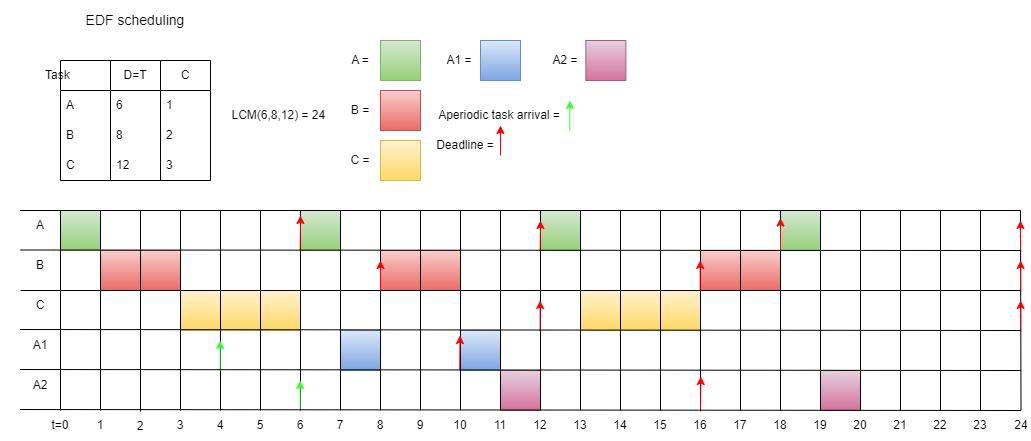
\includegraphics[width=0.8\textwidth]{images/Ass1Q8c.png}
            \caption{Tracing of the task set with soft aperiodic tasks A1 and A2. Both task A1 and A2 misses their deadlines, but since they are soft aperiodic tasks the deadline misses are not critical.}
            \label{fig:Q8trace}
        \end{figure}